\documentclass[times, utf8, zavrsni, numeric]{fer}
\usepackage{booktabs}
\usepackage{listings}
\usepackage{color}
\usepackage{url}
\usepackage{amsmath}

%Engleski termini
\newcommand{\eng}[1]{(eng. \textit{#1})}

\begin{document}

\title{ Lokalizacija karakterističnih točaka lica u videu }

\author{ \begin{tabular}{ l }
	Generalić Boris \\
	Gulan Filip \\
	Kopljar Damir \\
	Miličević Andrija \\
	Nuić Hrvoje \\
	Šarić Fredi \\
	Zadro Tvrtko \\
\end{tabular}  }

\maketitle
\tableofcontents

\chapter{Projektni zadatak}

\section{Opis projektnog zadatka}

Lokalizacija karakterističnih točaka lica u videu ili fotografiji je tehnika koja se danas koristi u mnogim sustavima i uređajima. Susrećemo je na raznim društvenim servisima, poput \textit{Facebook-a}, koji ju koriste za automatsko označavanje ljudi na fotografijama. Većina algoritama lokalizacije točaka lica su iznimno kompleksni i zahtijevaju veliku količinu procesorske snage i memorije, pa je težnja usmjerena na poboljšavanje tih algoritama. No razvojem i napretkom tehnologije algoritmi lokalizacije točaka lica se danas uspješno, bez velikih problema, izvode i na mobilnim uređajima koji ih koriste u raznoraznim aplikacijama poput alata za šminkanje gdje osoba može uz pomoć praćenja lica vidjeti kako bi izgledali s određenim bojama na svom licu.

Kroz ovaj projekt će se pokušati dani problem lokalizacije karakterističnih točaka lica riješiti uporabom dubokih neuronskih mreža.

\section{TODO: Pregled i opis srodnih rješenja}
\subsection{Xavier P. Burgos-Artizzu - Robust Cascaded Pose Regression}
RCPR metoda za detekciju karakterističnih točaka lica je poboljšanje metode CPR (\textit{Cascaded pose regression}). CPR metoda je vrlo efikasna i precizna u određivanju karakterističnih točaka lica, ali preciznost joj drastično opada kada se određuju karakteristične točke na licima koje su prekrivene s nekom preprekom. 

CPR uči kaskadu regresora R\textsuperscript{1\ldots T} koji progresivno transformiraju inicijalni skup karakterističnih točaka S\textsuperscript{0} u finalni odabira karakterističnih točaka S\textsuperscript{T}. Skup točaka S\textsuperscript{i} je definiran kao $ S_p^i = [x_p, y_p], p \in 1\ldots P$. Svaki od regresora $R^t$ producira pomak osnovne konfiguracije točaka $ \delta S^t$ koji se kombinira s ulazom tog regresora i stvara se ulaz u slijedeći regresor $S^t = S^{t-1} + \delta S^t$. 

RCPR metoda zahtijeva da označene karakteristične točke imaju informaciju o tome je li karakteristična točka prekrivena nekom zaprekom (naočale, ruka ...) ili ne. Time je definirana karakteristična točka kao $S_p^i = [x_p, y_p, v_p]$, gdje je $v_p$ realna vrijednost iz intervala $[0, 1]$.

Slika se podijeli u $3 \times 3$ polje. Svako polje ima informaciju o postotku prepreka unutar polja dobivenu kao procjena temeljena na $S^{t-1}$ karakterističnih točaka. U svakom koraku $t$ se uči $S_tot$ regresora koji se treniraju samo na 1 od 9 predefiniranih polja (svakom regresoru $R_i^t$ je nasumično dodijeljeno polje). Regresori generiraju pomake $\delta S_{1\ldots tot}$ iz kojih se računa težinski prosjek, gdje su težine obrnuto proporcionalne količini zapreka u polju na kojem je treniran regresor(za dobre rezultate dovoljno je koristiti $S_tot = 3$ regresora). Na kraju kaskade se dobiva finalni skup točaka $S_p^T = [x_p, y_p, v_p]$ te je potrebno odrediti prag $\tau$ koji označava je li točka $S_p$ prekrivena ili ne.

Metoda je testirana na tri različita skupa podataka (\textbf{LFPW}, \textbf{HELEN}, \textbf{LFW}) u kojima lica nisu prekrivena i postigla je bolje rezultate u odnosu na prijašnje metode, te je testirana na skupu podataka \textbf{COFW} u kojem su karakteristične točke lica djelomično prekrivene te je postigla zadovoljavajuće  rezultate.

\section{Konceptualno rješenje zadatka}

Sam sustav za lokalizaciju karakterističnih točaka lica je podijeljen u više segmenata, tj. podsustava. Prvi segment sustava na ulaz prima sliku ili jedan vremenski okvir video isječka. Dana slika ili isječak se zatim pretvaraju u sliku sivih nijansi. Tako obrađena slika se dovodi na ulaz podsustava za izlučivanje položaja svih lica na slici te kao rezultat vraća listu u obliku: koordinate gornjeg lijevog ugla, širina i visina lica.

Tako dobivena lista se zatim iskoristi na način da se iz slike sivih nijansi izrežu prepoznata lica i skaliraju. Pojedina skalirana lica dovede se na ulaze duboke neuronske mreže koja kao izlaze daje koordinate odabranih karakterističnih točaka lica. Tako dobivene točke skaliraju se u prostor početne slike ili isječka te se iscrtavaju i prikazuju korisniku sustava.

\chapter{Postupak rješavanja zadatka}

\section{Pretvorba boje u nijanse sive}

Prvi korak koji je potrebno napraviti na ulaznoj slici je pretvoriti ju u sliku sivih nijansi. Kod prikaza boja slike korištenjem aditivnog RGB \engl{Red Green Blue} modela postoje tri komponente: crvena, zelena i plava. Kombinacijom te tri komponente u različitim omjerima dobivamo ostale boje. Da se uočiti da podjednakom raspodjelom svih triju komponenti dobivamo boje iz sivog spektra, pa se algoritam pretvorbe u sliku sivih nijansi temelji na odabiru jedne vrijednosti iz dane tri komponente kako bi se dobila siva nijansa.

\subsection{Prvi algoritam}

Prvi algoritam je vrlo jednostavan i intuitivan. Siva nijansa pojedinog slikovnog elementa se dobiva tako da se boja slikovnog elementa rastavi na tri navedene komponente. Omjer pojedinih komponenti se zbraja te se uzima srednja vrijednost, kako je prikazano izrazom \eqref{eq:ug}.
\begin{equation}\label{eq:ug}
E_y = \frac{E_R + E_G + E_B}{3}
\end{equation} 

\subsection{Drugi algoritam}

Prvi algoritam je intuitivan i vrlo jednostavan, no u praksi ne daje najbolje rezultate. Problem leži u ljudskom oku i načinu na koji opaža boje. Ljudsko oko zelenu boju opaža puno jače nego crvenu, te crvenu opaža jače nego plavu. Stoga intuitivno slijedi da bi zelena trebala biti najzastupljenija, zatim crvena i plava. Organizacija ITU \engl{International Telecommunication Union} u svojoj normi ITU-R BT.709-6 \citep{ITUgrayscale} predlaže drugi algoritam u kojem bi crvena komponenta imala udio s 22.16\%, zelena s 71.56\% te plava s 7.22\%, što je prikazano izrazom \eqref{eq:itu_grayscale}.
\begin{equation} \label{eq:itu_grayscale}
E_y = 0.2126E_R + 0.7152E_G + 0.0722E_B
\end{equation}

Na slici \ref{fig:grayscale_example_all} mogu se usporediti rezultati obadva izraza, gdje je jasno vidljiva prednost korištenja izraza \eqref{eq:itu_grayscale}.

\begin{figure}[htb]
    \centering
    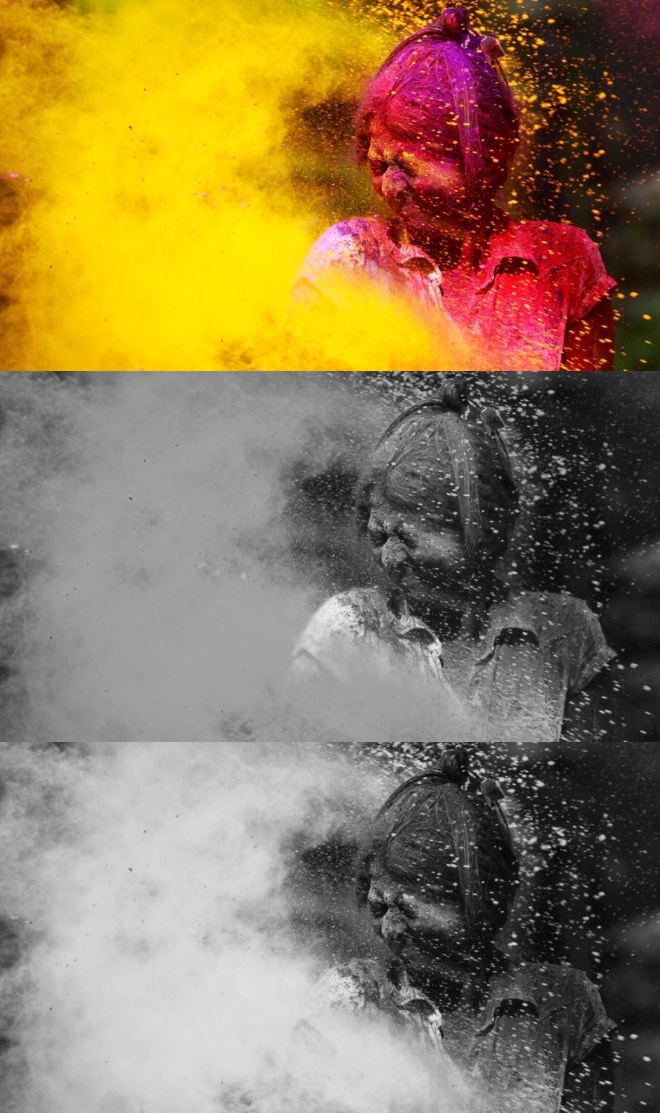
\includegraphics[width=9cm]{images/grayscale_example_all.jpg}
    \caption{Usporedba prvog i drugog algoritma pretvorbe boja u nijanse sive}
    \label{fig:grayscale_example_all}
\end{figure}

\section{Izjednačavanje histograma}

Nakon što je slika u boji pretvorena u sliku sivih nijansi vrlo lako je moguće da kontrast na danoj slici nije najbolji. U namjeri poboljšanja kontrasta na slici te izoštravanja pojedinih elemenata koristi se izjednačavanje histograma.

Izjednačavanje histograma slike je operacija pri kojoj se slika mijenja tako da broj točaka za pojedinu nijansu sive bude približno jednoliko raspoređen. Matematički rečeno izjednačavanje histograma implicira preslikavanje početne distribucije na širu i "uniformniju" distribuciju.

Kako je za potrebe ovog projekta korištena biblioteka \emph{OpenCV}, za izjednačavanje histograma korištena je metoda \emph{equalizeHist} iz navedene biblioteke. Primjer rada algoritma vidljiv je na slici \ref{fig:eq_hist}.

\begin{figure}[htb]
    \centering
    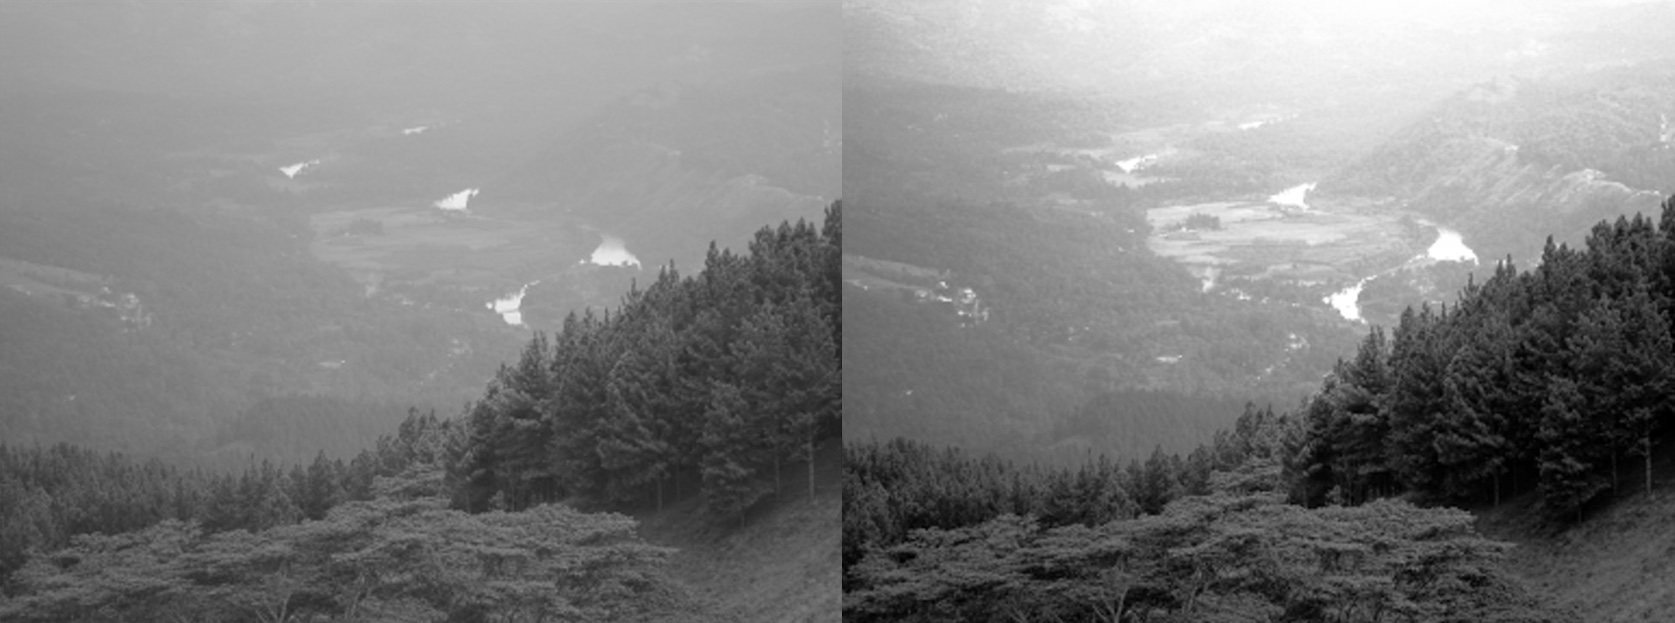
\includegraphics[width=14cm]{images/eq_hist.jpg}
    \caption{Izjednačavanje histograma}
    \label{fig:eq_hist}
\end{figure}

\section{Detekcija i izlučivanje lica}

Nakon što je slika u potpunosti obrađena slijedi detekcija, tj. izlučivanje pozicija lica na slici. Kako je za potrebe ovog projekta korištena biblioteka \emph{OpenCV}, za izlučivanje pozicije lica korištene korištene su kaskade boostanih Haarovih klasifikatora.

Metodu korištenja boostanih Haarovih klasifikatora predložili su Paul Viola i Michael Jones ne tako davne 2002. godine. To je ujedno bila prva metoda iz strojnog učenja koja postiže dobre rezultate u realnom vremenu. Iako je primarna svrha te metode prepoznavanje lica, može se iskoristiti za učenje prepoznavanja i ostalih objekata \citep{culjakRad}.

Metoda Viola-Jones umjesto direktnog rada s slikovnim elementima ulazne slike, što se pokazao kao proces s velikom složenošču, radi s određenim skupom reduciranih značajki te slike, to jest Haarovim značajkama. Haarove značajke su pravokutne značajke i računaju se kao razlika nekoliko suma slikovnih elemenata unutar različitih pravokutnih područja slike. Vrijednosti dobivene takvim računom predstavljaju prisustvo ili odsustvo nekih karakteristika slike (kao što su rubovi, kutevi i sl.) \citep{culjakRad}.

\begin{figure}[htb]
    \centering
    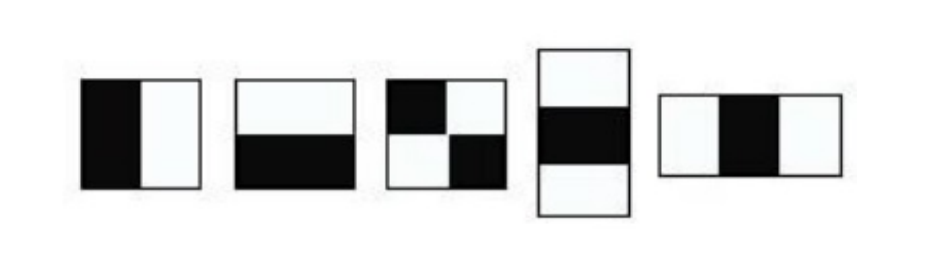
\includegraphics[width=12cm]{images/haar.png}
    \caption{Osnovne Haarove značajke}
    \label{fig:haar}
\end{figure}

Na slici \ref{fig:haar} prikazane su osnovne Haarove značajke. Skaliranjem, rotacijom i translacijom osnovnih značajki nastaju ostale Haarove značajke. Svaka značajka je konvolucijska maska, a vrijednost značajke, kako je već navedeno, dobiva se oduzimanjem sume vrijednosti slikovnih elemenata ispod bijelog područja od sume crnog područja pomnoženog s omjerom crne i bijele površine. Upravo zbog toga su te značajke vrlo osjetljive na promjenu kontrasta pa ih se interpretira kao značajke ruba ili linije \citep{franicRad}.

\begin{figure}[htb]
    \centering
    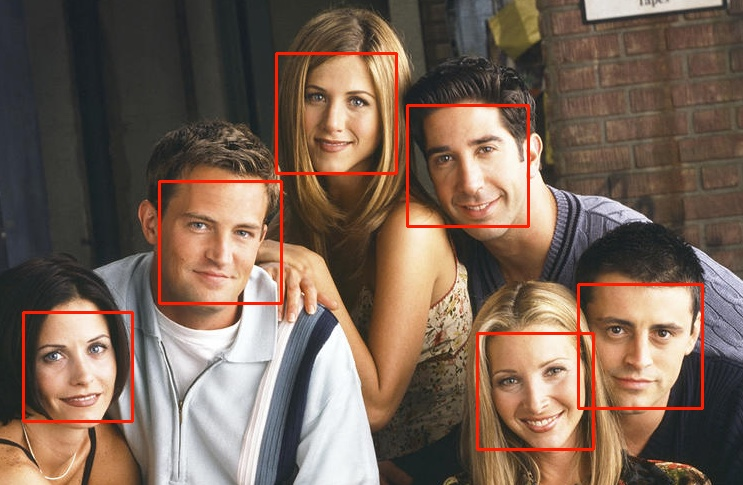
\includegraphics[width=13cm]{images/friends.jpg}
    \caption{Primjer rada kaskadnog Haarovog klasifikatora}
    \label{fig:haar_cls}
\end{figure}

\emph{CascadeClassifier} razred iz biblioteke \emph{OpenCV} u konstruktoru prima putanju do \emph{xml} datoteke koja sadrži naučenu kaskadu Haarovih klasifikatora. Za potrebe ovog rada korištena je datoteka \emph{haarcascade frontalface default} koja dolazi skupa s bibliotekom \emph{OpenCV}. Metoda \emph{detectMultiScale} prima na ulaz sliku sivih nijansi te vraća listu pozicija lica na slici. Primjer rada algoritma je vidljiv na slici \ref{fig:haar_cls}.

\section{Lokalizacija karakterističnih točaka lica}

Nakon izlučivanja pojedinih lica iz slike, dana lica se režu te skaliraju na uniformne vrijednosti, u ovom slučaju na dimenziju $96 \times 96$ slikovnih elemenata. Tako skalirana lica, tj. njihovi slikovni elementi se dovode na ulaze duboke neuronske mreže koja na svojim izlazima daje koordinate petnaest karakterističnih točaka lica: vrh nosa, lijevi i desni rub usta, sredina gornje i donje usne, centar oba oka, lijevi i desni kraj oba oka te lijevi i desni kraj obje obrve.

Primjer rada duboke neuronske mreže na lokalizaciji karakterističnih točaka lica vidljiv je na slici \ref{fig:lkt}.

\begin{figure}[htb]
    \centering
    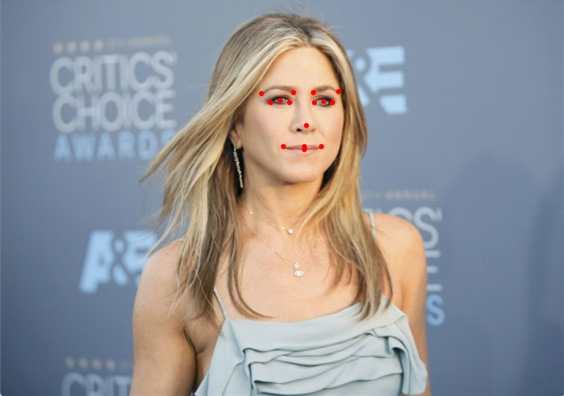
\includegraphics[width=13cm]{images/jennifer_good.jpg}
    \caption{Lokalizacija karakterističnih točaka lica}
    \label{fig:lkt}
\end{figure}

\subsection{TODO: Duboka neuronska mreža - Andrija ovdje ubaci teoriju}

\chapter{Ispitivanje rješenja}

\section{Ispitna baza}

Baza lica preuzeta je s jednog od natjecanja sa servisa \emph{Kaggle} \citep{kaggle}. Točnije, preuzeta je s natjecanja \emph{Facial Keypoints Detection} koje je otvoreno 2013. godine i zatvorilo se nedavno, početkom 2017. godine, za vrijeme pisanja ovog rada.

Dana baza se sastoji od 7049 označenih slika lica u skupu za učenje te 1783 neoznačenih slika u skupu za testiranje, odnosno u skupu koji se poglavito koristio za samu evaluaciju natjecanja. Svaka slika lica je dimenzija $96 \times 96$. Slike lica su označene sa 15 karakterističnih točaka:

\begin{itemize}
    \item vrh nosa, 
    \item lijevi i desni rub usta, 
    \item sredina gornje i donje usne, 
    \item centar oba oka,
    \item lijevi i desni kraj oba oka te 
    \item lijevi i desni kraj obje obrve.
\end{itemize}

Bitno je napomenuti da nisu svih 7049 slika lica iz skupa za učenje u potpunosti označene, već nekima nedostaju pojedine značajke. Stoga se broj iskoristivih slika za učenje smanjio na brojku nešto manju od 2200. No, za rješavanje tog problema iskorištena je metoda koja je predložena u članku \citep{daniel}. Dakle, svaka dostupna slika lica sa svim označenim značajkama je zrcaljena, kako je prikazano na slici \ref{fig:flip}, te na taj način se skup za učenje udvostručio i osigurana je bolja generalizacija neuronske mreže.

\begin{figure}[htb]
    \centering
    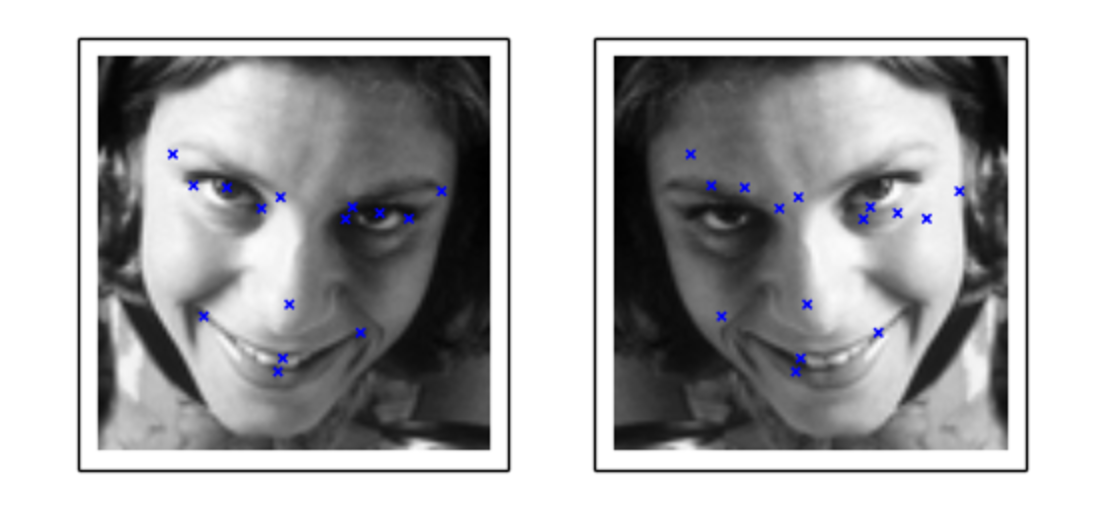
\includegraphics[width=12cm]{images/face_flip.png}
    \caption{Zrcaljeno lice}
    \label{fig:flip}
\end{figure}

\section{Rezultati učenja i ispitivanja}

Što se tiče samog učenja duboke neuronske mreže, ono je provedeno uporabom grafičke kartice. Kako je učenje duboke neuronske mreže uporabom običnog stolnoga računala, bez korištenja grafičke kartice, vrlo sporo bilo je nužno posegnuti za nešto kompliciranijim i skupljim metodama. Za potrebe ovog projekta na servisu \emph{Microsoft Azure} podignut je virtualni stroj s \emph{nVidia Tesla K80 24GB CUDA} grafičkom karticom koji je učenje mreže obavljao bez većih problema. Usporedbe radi, na stolnom računalu jedna epoha učenja duboke neuronske mreže je trajala oko 63 sekunde, dok je na virtualnom stroju to iznosilo oko 1.33 sekunde. Kako je mreža u ovom projektu učena i na više od $18.000$ epoha, razlika je bila više nego osjetna.

Prilikom učenja duboke neuronske mreže $30\%$ skupa za učenje je izuzeto kao skup za validaciju na kojem se provjeravala uspješnost generalizacija. Na grafu \ref{fig:lc} je prikazan odnos srednje kvadratne pogreške između skupa za validaciju i skupa za testiranje prilikom učenja. Tako naučena mreža je ostvarila minimalnu srednju pogrešku na skupu za učenje iznosa $0.00068$, te na skupu za validaciju iznosa $0.00072$.

\begin{figure}[htb]
    \centering
    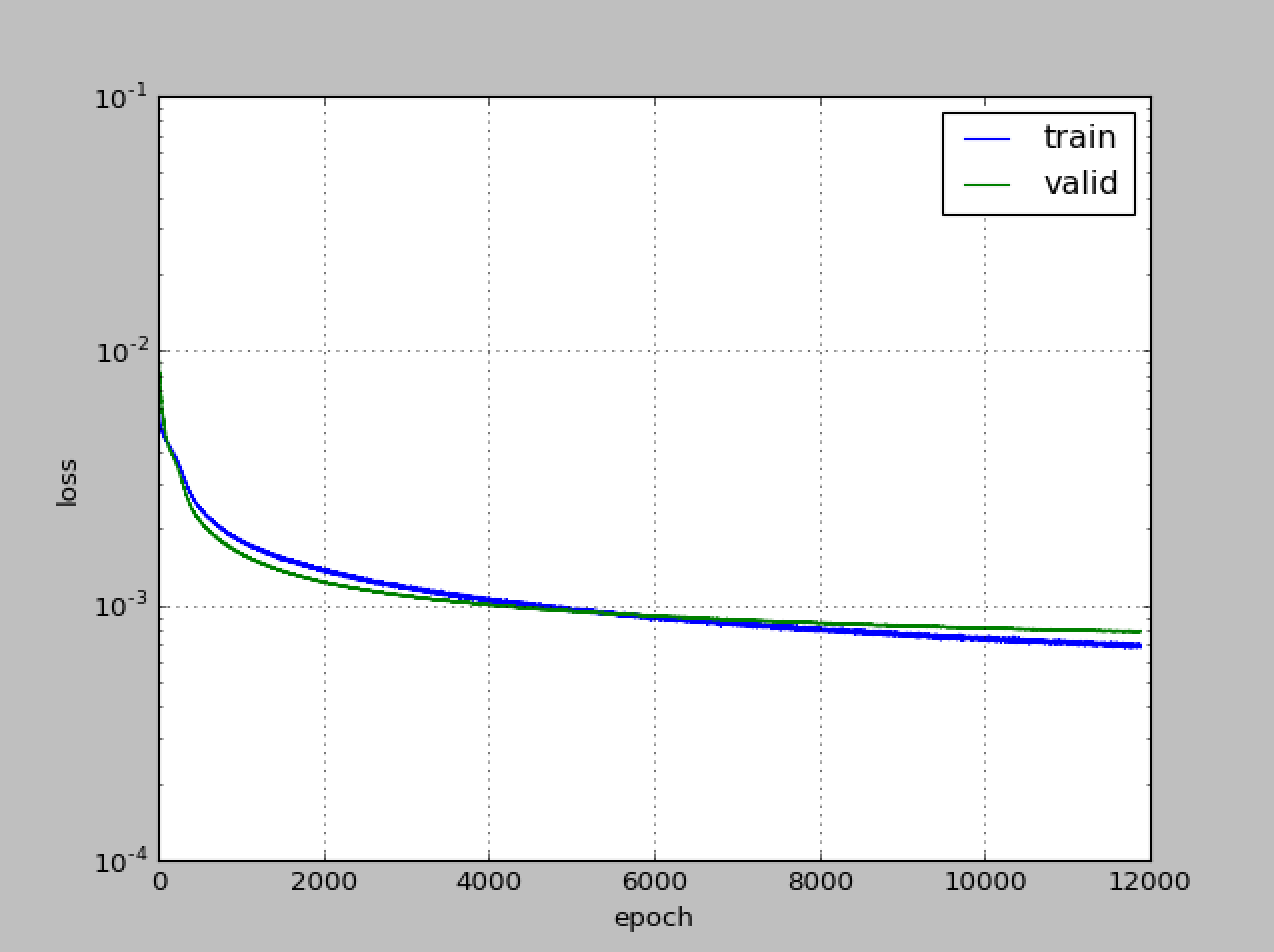
\includegraphics[width=14cm]{images/l_curves.png}
    \caption{Srednja kvadratna pogreška tokom učenja}
    \label{fig:lc}
\end{figure}

\chapter{Opis programske implementacije rješenja}

Programski kod korišten u ovome projektu napisan je u programskom jeziku Python (verzija 2.7.13). U projektu je korišteno nekoliko vanjskih biblioteka koje su potrebne za rad programa:
\begin{itemize}
    \item NumPy - rad s matricama,
    \item Scikit-learn - za učenje mreže,
    \item Theano - za učenje mreže kako na grafičkoj kartici tako i na procesoru,
    \item Matplotlib - prikaz grafova,
    \item Pandas - olakšan rad s korištenim strukturama,
    \item CUDA toolkit - za pristup i rad na grafičkoj kartici i
    \item OpenCV - biblioteka za prepoznavanje lica i rad s video zapisima.
\end{itemize}

Program se sastoji od 7 datoteka koje su potrebne za učenje i izvođenje programa.
Datoteke \emph{common.py}, \emph{tst\_scene\_render.py} i \emph{video.py} koriste se za podršku rada s kamerom.

Unutar datoteke \emph{learn.py} nalazi se implementacija koda koja uči mrežu, odnosno donosi predikcije za dani ulaz. Iako je većina parametara za trenutni problem dobro podešena, korisnik može mijenjati parametre mreže ili parametre algoritma učenja. Neki od parametara koje je moguće lako podesiti su broj filtara, veličinu filtra, \textit{dropout} stopu, broj neurona u skrivenom sloju, moment i stopu učenja ili broj epoha.

Parametre koje je potrebno podesiti su varijable \emph{FTRAIN} i \emph{FTEST}. Vrijednost varijable \emph{FTRAIN} potrebno je postaviti kao putanju do datoteke u kojoj se nalaze podaci za učenje. Vrijednost varijable \emph{FTEST} treba postaviti kao putanju do datoteke u kojoj se nalaze podaci za testiranje.

Unutar datoteke \emph{face\_points\_detector.py} nalazi se kod koji najprije poziva algoritam za prepoznavanje lica te zatim koristi sliku lica kao ulaz za implementirani algoritam koji prepoznaje karakteristične točke u licu.

Unutar datoteke \emph{facedetect.py} nalazi se glavna metoda koja pokreće sam program. Unutar nje potrebno je postaviti putanju do mreže koja će se koristi.

Program je moguće pokretati na dva načina. Prvi način poziva se kao: \emph{python facedetect.py} i na taj način program će koristiti kameru računala te će nad video-zapisom kojeg dobiva od kamere pokretati predikciju karakterističnih točaka. Drugi način poziva se kao: \emph{python facedetect.py putanjaDoSlike}, gdje \emph{putanjaDoSlike} predstavlja stvarnu putanju do slike, koja će se koristi kao ulaz za predikciju karakterističnih točaka lica na slici.

\chapter{Zaključak}

Duboka neuronska mreža se pokazala kao dobar model za rješavanje problema lokalizacije karakterističnih točaka lica. Unatoč lošijim performanse na običnim stolnim računalima prilikom samog učenja, sama mreža nije predstavljala usko grlo sustava prilikom samog iskorištavanja za lokalizaciju točaka.

Daljnja poboljšanja se mogu ostvariti u vidu nešto boljeg i većeg skupa podataka. Uočeno je nekoliko problema sa samo mrežom za koje je većinom odgovoran skup podataka za učenje. Na primjer, mreža teško prati jako otvorena usta, čisto iz razloga jer takvih primjera slika nema u skupu za učenje. Također ima problema s praćenjem visoko podignutih obrva, iz istog razloga kao i s ustima.

Što se tiče samog sustava kao cjeline problem predstavlja nerobusnost Haarovih kaskadnih klasifikatora prilikom lokalizacije lica te bi se u budućim radovima trebalo posvetiti i tom problemu. Navedeni kaskadni klasifikatori jako teško detektiraju lice ukoliko je osoba malo nakrivila ili zakrenula glavu.

\bibliography{literatura}
\bibliographystyle{fer}

\end{document}
